\documentclass[12pt]{article}
\usepackage[a4paper, lmargin=1in, rmargin=1in, tmargin=1in, bmargin=1in]{geometry}
\usepackage{amsfonts}
\usepackage{amsmath}
\usepackage{mathtools}
\usepackage{calc}
\usepackage{amssymb}
\usepackage{multicol}
\usepackage{xparse}
\usepackage{icomma}
\usepackage[a]{esvect}
\usepackage{graphicx}
\usepackage{enumitem}
\usepackage{fancyhdr}
\usepackage{parskip}
\usepackage{indentfirst}
\usepackage{gensymb}
\usepackage{mdframed}
\usepackage{pdfpages}
\usepackage{tikz}
\usepackage{bm}
\usepackage{color}
\usepackage{cancel}
\usepackage{pgfplots}
\usepackage{colortbl}
\usepackage{etex}
\usepackage{tkz-euclide}

%% Impor library tikz %%
\usetikzlibrary{shapes}
\usetikzlibrary{arrows}
\usetikzlibrary{calc}
\usetikzlibrary{through}
\usetikzlibrary{intersections}
\usetikzlibrary{math}
\usetikzlibrary{angles}
\usetikzlibrary{positioning}
\usetikzlibrary{quotes}
\usetikzlibrary{decorations.markings}

%% Buat command baru untuk membuat simbol diferensial %%
\newcommand*\diff{\mathop{}\!\mathrm{d}}

%% Setel panjang indentasi %%
\setlength{\parindent}{5ex}

%% Ganti simbol himpunan kosong dengan varnothing %%
\let\oldemptyset\emptyset
\let\emptyset\varnothing

%% Buat beberapa fitur otomatis untuk menambahkan bar %%
\newcommand*\norm[1]{\mathop{}\!\left\|#1\right\|}
\newcommand*\lrbr[1]{\mathop{}\!\left\lbrace#1\right\rbrace}
\newcommand*\lrag[1]{\mathop{}\!\left\langle{#1}\right\rangle}
\newcommand*\lbrk[1]{\mathop{}\!\left({#1}\right]}
\newcommand*\lkrb[1]{\mathop{}\!\left[{#1}\right)}
\newcommand*\floor[1]{\mathop{}\!\left\lfloor{#1}\right\rfloor}
\newcommand*\ceil[1]{\mathop{}\!\left\lceil{#1}\right\rceil}
\newcommand*\func[2]{\mathop{}\!{#1}{\left({#2}\right)}}
\newcommand*\funk[2]{\mathop{}\!{#1}{\left[{#2}\right]}}
\newcommand*\funl[2]{\mathop{}\!{#1}{\left\lbrace{#2}\right\rbrace}}
\newcommand*\funa[2]{\mathop{}\!{#1}{\left|{#2}\right|}}
\newcommand*\set[2]{\mathop{}\!\left\lbrace{{#1} \, \left| \, {#2} \right.}\right\rbrace}

%% Buat underbrace agar dapat berada pada notasi matematika %%
\newcommand*\ubr[2]{\mathop{}\!\underbrace{#1}_{\text{$ {#2} $}}}

%% Buat tanda titik-titik vertikal dan membuat tanda tersebut tepat ditengah-tengah tanda sama dengan %%
%% Biasanya digunakan untuk membuat persamaan yang memiliki algoritma sama %%
\newcommand*\cvdot[1]{\mathop{}\!\mathrel{\makebox[\widthof{$ {#1} $}]{\vdots}}}

%% Item default untuk environment enumerate %%
\newcommand\defitem{\item[$ \bullet $]}

%% Ganti notasi logaritma dengan varlog %%
\let\oldlog\log
\let\log\varlog

%% Ganti syntax displaystyle menjadi ds agar lebih mudah %%
\newcommand*\ds[1]{\mathop{}\!\displaystyle{{#1}}}

%% Definisi varlog %%
%% Perbedaan notasi logaritma ini dengan notasi logaritma awal (yang diganti) berada pada basis logaritmanya %%
%% Notasi baru ini menggunakan basis logaritma yang digunakan di Indonesia (sebagai ganti dari notasi logaritma internasional) %%
\NewDocumentCommand{\log}{o}
{
	\IfNoValueTF{#1}
	{}
	{{}^{{#1}}\!}
	\oldlog
}

%% Buat tambahan operator matematika %%
\DeclareMathOperator{\sgn}{sgn}				% signum
\DeclareMathOperator{\csch}{csch}			% kosekan hiperbolik
\DeclareMathOperator{\sech}{sech}			% sekan hiperbolik
\DeclareMathOperator{\arcsec}{arcsec}		% sekan invers
\DeclareMathOperator{\arccsc}{arccsc}		% kosekan invers
\DeclareMathOperator{\arccot}{arccot}		% kotangen invers
\DeclareMathOperator{\lcm}{lcm}				% least common multiple (kelipatan persekutuan terbesar)
\DeclareMathOperator{\arsinh}{arsinh}		% sinus hiperbolik invers
\DeclareMathOperator{\arcosh}{arcosh}		% kosinus hiperbolik invers
\DeclareMathOperator{\artanh}{artanh}		% tangen hiperbolik invers
\DeclareMathOperator{\arcsch}{arcsch}		% kosekan hiperbolik invers
\DeclareMathOperator{\arsech}{arsech}		% sekan hiperbolik invers
\DeclareMathOperator{\arcoth}{arcoth}		% kotangen hiperbolik invers

%% Buat fitur satuan untuk suatu besaran fisis %%
\newcommand*\punit[1]{\mathop{}\!\, \mathrm{{#1}}}

%% Buat notasi-notasi yang menggunakan teks roman %%
\newcommand*{\transpose}{\mathop{}\!\mathrm{T}}
\newcommand*{\comp}{\mathop{}\!\mathrm{C}}

%% Buat notasi turunan pada suatu titik %%
\newcommand{\at}[2][]{#1|_{#2}}

%% Buat warna untuk membedakan pencoretan %%
\newcommand\ccancel[2][black]{\renewcommand\CancelColor{\color{#1}}\cancel{#2}}

%% Buat header dan footer untuk dokumen %%
\pagestyle{fancy}
\lfoot{Made with \LaTeX}
\cfoot{\thepage}
\rfoot{\copyright \, Pak Angga, \the\year}
\renewcommand{\headrulewidth}{0pt}
\renewcommand{\footrulewidth}{1pt}

\begin{document}
	%% Header &&
	\begin{center}
		{\large{\sc{
			Universitas Mulawarman \\
			Fakultas Keguruan dan Ilmu Pendidikan \\
			Pendidikan Matematika \\[3pt]
			Bank Soal HOTS Kalkulus I
		}}}
	\end{center}
	
	\vspace{5pt}
	
	\noindent Nama : \dotfill
	
	\vspace{-13pt}
	
	\noindent \hrulefill
	
	\vspace{5pt}
	
	%% Content %%
	\noindent \textbf{A. Limit}
	\begin{enumerate}[leftmargin=*]
		\item Tentukan nilai dari $ \ds{\lim_{x \to 0}{\frac{\sqrt{1 - \func{\cos^{2}}{x}}}{x}}} $.
		\item Tentukan nilai dari $ \ds{\lim_{x \to 0}{\frac{\left|x + 1\right| - \left|x - 1\right|}{x}}} $.
		\item Gunakan lingkaran satuan untuk menunjukkan bahwa
		\[ \func{\sin^{2}}{\theta} \leq \left(1 - \func{\cos}{\theta}\right)^{2} + \func{\sin^{2}}{\theta} \leq \theta^{2}. \]
		Kemudian dengan menggunakan hasil yang telah Anda buktikan sebelumnya, buktikan bahwa
		\[ \lim_{\theta \to 0}{\frac{1 - \func{\cos}{\theta}}{\theta^{2}}} = \frac{1}{2}. \]
		\item Hitung limit-limit berikut.
		\begin{enumerate}
			\item $ \ds{\lim_{x \to \infty}{x\func{\sin}{\frac{1}{x}}}} $
			\item $ \ds{\lim_{x \to \pi}{\frac{\pi - x}{\func{\sin}{x}}}} $
			\item $ \ds{\lim_{x \to 2}{\frac{\func{\cos}{\dfrac{\pi}{x}}}{x - 2}}} $
		\end{enumerate}
		\item Hitung limit berikut atau berikan alasan mengapa limitnya tidak ada.
		\begin{enumerate}
			\item $ \ds{\lim_{x \to 0}{\frac{x^{2}\left(1 + \func{\sin^{2}}{x}\right)}{\left(x + \func{\sin}{x}\right)^{2}}}} $
			\item $ \ds{\lim_{x \to \infty}{\frac{x^{2}\left(1 + \func{\sin^{2}}{x}\right)}{\left(x + \func{\sin}{x}\right)^{2}}}} $
		\end{enumerate}
		\item Diketahui $ \func{f}{x} = ax^{2} + b $. Jika $ \func{f}{2b} - \func{f}{b} = 3 $ dan $ \ds{\lim_{x \to 1}{\frac{\func{f}{bx}}{x - 1}}} = 2 $, maka tentukan nilai dari $ a + b $.
		\item Tentukan nilai dari $ \ds{\lim_{x \to \infty}{2x\func{\tan}{\frac{1}{x}}\func{\sec}{\frac{2}{x}}}} $.
		\item Tentukan nilai dari
		\[ \func{\lim_{x \to 1}}{\left(\frac{4}{x^{2} - x} - \frac{x^{2} - 3x + 4}{1 - x^{3}}\right)^{-1} + \frac{4\left(x^{4} - 1\right)}{x^{2} - \dfrac{1}{x}}}. \]
		\item Jika konstanta $ a $ dan $ b $ memenuhi $ \ds{\lim_{x \to 1}{\frac{x - 1}{\sqrt{x + a} + b}}} = 4 $, maka tentukan nilai dari $ a + b $.
		\item Misalkan $ f : \mathbb{R} \to \mathbb{R} $ fungsi kontinu. Asumsikan untuk sebarang $ c > 0 $, grafik fungsi $ f $ dapat dipindahkan ke grafik fungsi $ cf $ hanya dengan menggunakan translasi dan rotasi. Apakah ini mengimplikasikan $ \func{f}{x} = ax + b $ untuk suatu bilangan real $ a $ dan $ b $?
		\item Diberikan fungsi $ f, g : \mathbb{R} \to \mathbb{R} $ yang memenuhi $ \func{g}{x} = \func{f}{2ax} $ untuk setiap bilangan real $ x $ dan $ a > 0 $. Jika $ \ds{\lim_{x \to 0}{\func{f}{x}}} = \ell $, maka tentukan nilai dari $ \ds{\lim_{x \to 0}{\func{g}{x}}} $.
		\item Misalkan $ f $ kontinu pada $ \left[a, b\right] $ dan tidak pernah bernilai nol pada selang tersebut. Apakah mungkin bahwa $ f $ berganti tanda pada $ \left[a, b\right] $?
		\item Misalkan fungsi $ f $ dan $ g $ memiliki limit di $ c \in \mathbb{R} $. Dengan menggunakan definisi limit, buktikan bahwa $ \ds{\lim_{x \to c}{\func{f}{x}\func{g}{x}}} = \ds{\lim_{x \to c}{\func{f}{x}}}\ds{\lim_{x \to c}{\func{g}{x}}} $.
		\item Diberikan titik-titik pada bidang koordinat $ M\left(1, 0\right) $, $ N\left(0, 1\right) $, $ O\left(0, 0\right) $, dan $ P\left(x, y\right) $ pada grafik $ y = \sqrt{x} $. Tentukan nilai dari
		\[ \lim_{x \to 0^{+}}{\frac{\left[NOP\right]}{\left[MOP\right]}}. \]
		\item Untuk sebarang bilangan real $ \alpha $, notasi $ \floor{\alpha} $ menyatakan bilangan bulat terbesar yang lebih kecil atau sama dengan $ \alpha $. Hitunglah nilai dari $ \ds{\lim_{x \to 0}{x\floor{\frac{1}{x}}}} $.
		\item Untuk setiap bilangan bulat positif $ n $, misalkan $ S_{n} $ dinotasikan sebagai panjang total interval $ x $ yang memenuhi $ \func{\sin}{4x} \geq \func{\sin}{x} $ pada $ 0 \leq x \leq 2\pi $. Tentukanlah nilai dari $ \displaystyle{\lim_{n \to \infty}{S_{n}}} $.
		\item Tentukan nilai dari
		\[ \lim_{x \to \infty}{\left(\sqrt[3]{8x^{3} + 48x^{2} + 96x - 2019} + \sqrt[4]{81x^{4} + 2020} - 5x - 2021\right)}. \]
		\item Suatu koin tak seimbang memiliki peluang sebesar $ t $ dengan $ 0 < t < \dfrac{1}{2} $ untuk mendapatkan sisi gambar ketika mendarat setelah dilemparkan dan memiliki peluang sebesar $ 1 - t $ untuk mendapatkan sisi angka. Koin ini dilemparkan sebanyak $ n $ kali dengan $ n \geq 2 $. Notasikan $ A_{n} $ sebagai kejadian bahwa sisi gambar muncul setidaknya dua kali dalam $ n $ kali pelemparan dan notasikan $ B_{n} $ sebagai kejadian bahwa sisi gambar tidak akan muncul setelah sisi angka hingga percobaan ke-$ n $. Jika $ \func{P}{X} $ dinotasikan sebagai peluang terjadinya suatu kejadian $ X $, tentukanlah nilai dari
		\[ \lim_{n \to \infty}{\frac{\func{P}{A_{n}}\func{P}{B_{n}}}{\func{P}{A_{n} \cap B_{n}}}}. \]
		\item Mulai pukul empat pagi, seorang pejalan kaki secara perlahan mendaki ke puncak gunung dan tiba pada tengah hari. Keesokan harinya dia turun kembali dengan menelusuri jalan yang sama, mulai pukul lima pagi dan tiba di bawah pada pukul sebelas pagi. Tunjukkan bahwa pada suatu titik di sepanjang jalan, jam tangannya menunjukkan waktu yang sama pada kedua hari itu.
		\item Misalkan $ \func{f}{x + y} = \func{f}{x} + \func{f}{y} $ untuk semua bilangan real $ x $ dan $ y $. Jika $ f $ kontinu di $ x = 0 $, buktikan bahwa $ f $ juga kontinu dimana-mana.
		\item Tentukan nilai dari $ \ds{\lim_{n \to \infty}{\sqrt[n]{n}}} $.
		\item Diberikan bilangan real positif $ a < 1 $. Buktikan bahwa $ \ds{\lim_{n \to \infty}{a^{n}}} = 0 $.
		\item Buktikan bahwa $ \ds{\lim_{n \to \infty}{\left(-1\right)^{n}}} $ tidak ada.
		\item Buktikan ketunggalan limit. Artinya, buktikan bahwa untuk setiap bilangan real $ c $, jika $ \ds{\lim_{x \to c}{\func{f}{x}}} = L_{1} $ dan $ \ds{\lim_{x \to c}{\func{f}{x}}} = L_{2} $, maka $ L_{1} = L_{2} $.
		\item Diberikan bilangan bulat $ n $. Misalkan $ \func{M}{n} $ bilangan bulat terbesar $ m $ sedemikian sehingga
		\[ \binom{m}{n - 1} > \binom{m - 1}{n}. \]
		Hitunglah nilai dari
		\[ \lim_{n \to \infty}{\frac{\func{M}{n}}{n}}. \]
		\item Diberikan segitiga siku-siku $ ABC $ yang siku-siku di titik $ C $ dan $ \angle{BAC} = \theta $. Titik $ D $ dipilih pada $ \overline{AB} $ sedemikian sehingga $ \left|AC\right| = \left|AD\right| = 1 $. Titik $ E $ dipilih pada $ BC $ sedemikian sehingga $ \angle{CDE} = \theta $. Garis tegak lurus dari $ E $ memotong $ AB $ di $ F $. Tentukan nilai dari $ \displaystyle{\lim_{\theta \to 0}{\left|EF\right|}} $.
		\item Diberikan segitiga sebarang $ ABC $ dengan $ \angle{ABC} = 110^{\circ} $. Diketahui $ \left|AB\right| = 1 $. Begitu $ \overline{BC} $ dan $ \overline{AC} $ meningkat, panjang $ \overline{AB} $ tetap 1 dan $ \angle{ABC} $ tetap $ 110^{\circ} $. Tentukan nilai dari
		\[ \lim_{\substack{\left|AC\right| \to \infty \\ \left|BC\right| \to \infty}}{\left(\left|AC\right| - \left|BC\right|\right)}. \]
		\item Jika $ \ds{\lim_{x \to c}{\frac{1}{\left(x - c\right)^{n}}\sum_{k = 0}^{n}{a_{k}\left(x - c\right)^{k}}}} = 0 $, maka tentukanlah nilai dari $ a_{0} + a_{1} + \cdots + a_{n} $.
		\item Diketahui $ a \in \mathbb{R} $ dan fungsi $ f : \mathbb{R} \to \mathbb{R} $ memenuhi $ \left|x\func{f}{x} + a\right| < \func{\sin^{2}}{x - a} $ untuk setiap bilangan real $ x $. Tentukan nilai dari $ \ds{\lim_{x \to a}{\func{f}{x}}} $.
		\item Diketahui fungsi $ f : \left[0, 1\right] \to \mathbb{R} $ kontinu. Jika $ \func{f}{x} $ rasional untuk setiap $ x \in \left[0, 1\right] $ dan $ \func{f}{0} = 0 $, maka tentukan nilai dari $ \func{f}{\dfrac{\sqrt{2}}{4}} $.
		\item Diketahui fungsi $ f : \left(a, b\right) \to \mathbb{R} $ merupakan fungsi kontinu dengan $ \func{f}{r + \dfrac{1}{n}} = \func{f}{r} $ untuk setiap bilangan rasional $ r $ dan bilangan asli $ n $. Untuk setiap bilangan real $ x $, tentukan semua fungsi $ \func{f}{x} $ yang memenuhi.
		\item Misalkan $ f : \left(0, 1\right) \to \mathbb{R} $. Jika $ \ds{\lim_{x \to 0}{\func{f}{x}}} = 0 $ dan $ \ds{\lim_{x \to 0}{\frac{\func{f}{x} - \func{f}{x/2}}{x}}} = 0 $, tentukan nilai dari $ \ds{\lim_{x \to 0}{\frac{\func{f}{x}}{x}}} $.
		\item Buktikan bahwa tidak ada fungsi $ f $ yang kontinu pada himpunan bilangan real dan $ \func{f}{x} = c $ mempunyai tepat dua solusi untuk setiap bilangan real $ c $.
		\item Misalkan $ f $ dan $ g $ fungsi yang bernilai real pada garis bilangan real dan $ \func{f}{r} \leq \func{g}{r} $ untuk setiap bilangan rasional $ r $. Jika $ f $ dan $ g $ keduanya kontinu, apakah berlaku $ \func{f}{x} \leq \func{g}{x} $ untuk setiap bilangan real $ x $?
		\item Cari semua fungsi kontinu $ f : \mathbb{R} \to \mathbb{R} $ sedemikian sehingga $ \func{f}{x} - \func{f}{y} $ rasional untuk setiap bilangan real $ x $ dan $ y $ yang memenuhi $ x - y $ rasional.
		\item Cari semua fungsi $ f : \mathbb{R} \to \mathbb{R} $ sedemikian sehingga untuk setiap $ x, y \in \mathbb{R} $ berlaku
		\[ \func{f}{x + y} + \func{f}{x - y} = 2\func{f}{x}\func{f}{y} \quad \mbox{dan} \quad \lim_{x \to \infty}{\func{f}{x}} = 0. \]
		\item* Tunjukkan bahwa fungsi
		\[
			\func{f}{x}	=	\begin{cases}
								\hfil x,	& x \, \mbox{rasional} \\
								-x,			& x \, \mbox{irasional}
							\end{cases}
		\]
		kontinu hanya di $ x = 0 $.
		\item* Fungsi Thomae $ \func{T}{x} $ adalah fungsi yang didefinisikan sebagai
		\[
			\func{T}{x} \coloneqq	\begin{cases}
										\dfrac{1}{q}	& \text{jika }x=\dfrac{p}{q}\quad (x \text{ rasional), dengan } p \in \mathbb{Z} \text{ dan } q \in \mathbb{N} \text{ relatif prima} \\
										0				& \text{jika }x\text{ irasional.}
								\end{cases}.
		\]
		Buktikan bahwa fungsi Thomae kontinu hanya untuk setiap bilangan irasional $ x $.
		\item* Untuk setiap bilangan bulat $ n \geq 1 $, misalkan
		\[ a_{n} = \sum_{k = 1}^{n - 1}{\frac{\func{\sin}{\dfrac{2k - 1}{2n}\pi}}{\func{\cos^{2}}{\dfrac{k - 1}{2n}\pi}\func{\cos^{2}}{\dfrac{k}{2n}\pi}}}. \]
		Carilah nilai dari
		\[ \lim_{n \to \infty}{\frac{a_{n}}{n^{3}}}. \]
		\item* Tinjau suatu barisan
		\[ \left(a_{n}\right)_{n = 1}^{\infty} = \left(1, 1, 2, 1, 2, 3, 1, 2, 3, 4, 1, 2, 3, 4, 5, 1, \dots\right). \]
		Cari semua pasangan bilangan real positif $ \left(\alpha, \beta\right) $ sedemikian sehingga
		\[ \lim_{n \to \infty}{\frac{1}{n^{\alpha}}\sum_{k = 1}^{n}{a_{k}}} = \beta. \]
		\item* Diberikan barisan bilangan real $ x_{1}, x_{2}, x_{3}, \dots $ yang memenuhi $ x_{1} = \sqrt{5} $ dan $ x_{n + 1} = x_{n}^{2} - 2 $ untuk setiap $ n \geq 1 $. Hitunglah nilai dari
		\[ \lim_{n \to +\infty}{\frac{x_{1}x_{2}x_{3} \cdots x_{n}}{x_{n + 1}}}. \]
		\item* Untuk setiap bilangan real $ x $, notasi $ \floor{x} $ menyatakan bilangan bulat terbesar yang tidak lebih besar daripada $ x $. Tentukan semua polinomial dengan koefisien bilangan real $ \func{P}{x} $ yang memenuhi
		\[ \func{P}{\floor{x}} = \floor{\func{P}{x}} \]
		untuk setiap bilangan real $ x $.
		\item** Danu sedang sarapan pagi untuk mempersiapkan diri mengikuti perkuliahan. Ia mengambil sepotong roti dengan irisan daging diatasnya. Tunjukkan bahwa ada suatu garis sehingga jika Danu memotong roti-daging mengikuti garis tersebut menjadi dua bagian, maka masing-masing bagian mengandung roti dan daging sama banyak. \\
		\textit{Petunjuk: Pertama-tama tunjukkan bahwa untuk setiap sudut $ \theta $ yang dibentuk oleh irisan dan sumbu-$ x $ terdapat garis $ \func{L}{\theta} $ yang membagi dua roti (saja) sama besar.}
		\item** Bilangan bulat positif $ n $ dikatakan \textit{kuratis} apabila $ n $ merupakan kuadrat sempurna atau jarak dari $ n $ ke bilangan kuadrat sempurna terdekat juga merupakan bilangan kuadrat sempurna. Sebagai contoh, 21 adalah bilangan kuratis karena bilangan kuadrat sempurna terdekat dari 21 adalah $ 5^{2} = 25 $ dan $ 25 - 21 = 4 $ merupakan bilangan kuadrat sempurna. Untuk suatu bilangan bulat positif $ N $, misalkan $ \func{\sigma}{N} $ dinotasikan sebagai banyaknya bilangan kuratis antara 1 dan $ N $ secara inklusif. Cari konstanta positif $ \alpha $ dan $ \gamma $ sedemikian sehingga
		\[ \lim_{N \to \infty}{\frac{\func{\sigma}{N}}{N^{\alpha}}} = \gamma, \]
		atau tunjukkan bahwa konstanta yang dimaksud tidak ada.
		\item** Misalkan $ f : \left[-1, 1\right] \to \mathbb{R} $ fungsi kontinu sedemikian sehingga
		\begin{enumerate}
			\item[(i)] $ \func{f}{x} = \dfrac{2 - x^{2}}{2}\func{f}{\dfrac{x^{2}}{2 - x^{2}}} $ untuk setiap $ x \in \left[-1, 1\right] $;
			\item[(ii)] $ \func{f}{0} = 1 $; dan
			\item[(iii)] $ \ds{\lim_{x \to 1^{-}}{\frac{\func{f}{x}}{\sqrt{1 - x}}}} $ ada dan berhingga.
		\end{enumerate}
		Buktikan bahwa $ f $ tunggal dan ekspresikan $ \func{f}{x} $ dalam bentuk tertutup.
		\item** Misalkan $ \func{f}{x} $ fungsi kontinu yang memenuhi $ \func{f}{2x^{2} - 1} = 2x\func{f}{x} $ untuk setiap $ x $ yang berada pada domain fungsi $ f $. Buktikan bahwa $ \func{f}{x} = 0 $ untuk $ -1 \leq x \leq 1 $.
		\item** Diberikan konstanta $ c \geq 0 $. Tentukan semua fungsi kontinu $ f : \mathbb{R} \to \mathbb{R} $ yang memenuhi $ \func{f}{x} = \func{f}{x^{2} + c} $ untuk setiap bilangan real $ x $.
	\end{enumerate}
	
	\newpage
	
	\noindent \textbf{B. Turunan dan Antiturunan}
	\begin{enumerate}[leftmargin=*]
		\item Diketahui $ \func{f}{0} = 1 $ dan $ \func{f^{\prime}}{0} = 2 $. Jika $ \func{g}{x} = \dfrac{1}{\left(2\func{f}{x} - 1\right)^{2}} $, tentukan nilai dari $ \func{g^{\prime}}{0} $.
		\item Tentukan $ \ds{\int{\func{\cos^{2}}{x} \diff{x}}} - \ds{\int{\left(1 - \func{\sin^{2}}{x}\right) \diff{x}}} $.
		\item Misalkan $ S $ himpunan titik-titik dimana fungsi real $ \func{f}{x} = \left|2 - \left|x - 3\right|\right| $ tak terturunkan. Tentukan nilai dari
		\[ \sum_{x \in S}{\func{\left(f \circ f\right)}{x}}. \]
		\item Pemerintah daerah Kota Bontang berencana akan membuat rumah tahanan (rutan). Rutan tersebut terdiri dari 5 blok dan setiap bloknya terdiri dari tiga sel penjara yang berdampingan. Tepi kanan dan tepi kiri setiap blok dibatasi oleh tembok. Begitu juga dengan bagian belakang bloknya. Pemerintah Kota Bontang menginginkan setiap sel penjara memiliki jeruji besi yang berkualitas, namun harganya terjangkau. Setelah proses pencarian jeruji besi, didapatkan jeruji besi yang dijual seharga Rp2.500.000,00 per meternya. Asumsikan setiap sel penjara memiliki panjang dan lebar yang sama. Jika masing-masing sel penjara direncanakan memiliki luas $ 30 m^{2} $, tentukan panjang dan lebar setiap sel penjara agar biaya total pemasangan jeruji besi di rutan tersebut seminimum mungkin. Tentukan juga berapa biaya totalnya.
		\item Diketahui $ \func{f}{\dfrac{x - 1}{2x + 3}} = x^{2} - 4x + 3 $. Tentukan nilai dari $ \func{f^{\prime}}{0} $.
		\item Diketahui $ \func{f}{x + y} = \func{f}{x} + \func{f}{y} + x^{2}y - 4xy^{2} $ dan $ \displaystyle{\lim_{x \to 0}{\frac{\func{f}{x}}{x}} = 0} $. Tentukan bilangan real positif $ a $ yang memenuhi $ \func{f^{\prime}}{a} = 2021 $.
		\item Diketahui fungsi $ f, g : \mathbb{R} \to \mathbb{R} $ dengan $ \func{f}{x} = \begin{cases}
			ax + b, & x \leq \pi \\
			\func{\sin}{x}, & x > \pi
		\end{cases} $ dan $ \func{g}{x} = x - 1 $. Jika fungsi $ \func{f}{x} $ terturunkan dimana-mana, tentukanlah nilai dari $ \func{\left(f \circ g\right)}{\pi} $.
		\item Jika $ f : \mathbb{R} \to \mathbb{R} $ dengan $ \func{f}{x} = \begin{cases}
			\dfrac{\func{\sin}{x}}{x}, & x \ne 0 \\[2pt]
			1, & x = 0
		\end{cases} $, tentukan turunan pertama dari $ f $ dan buktikan bahwa $ f^{\prime} $ kontinu di 0.
		\item Diberikan $ f : \left(0, +\infty\right) $ mempunyai turunan dan $ \ds{\lim_{x \to \infty}{\func{f^{\prime}}{x}}} = 1 $. Jika $ \func{g}{x} = \func{f}{x + 1} - \func{f}{x} $, maka tentukan nilai dari $ \ds{\lim_{x \to \infty}{\func{g}{x}}} $.
		\item Misalkan $ \func{f}{x} $ fungsi real yang terturunkan sedemikian sehingga
		\[ \func{f^{\prime}}{x} = \func{f}{x}\func{f}{x}\func{f}{x}\cdots. \]
		Tentukan banyaknya fungsi $ \func{f}{x} $ yang memenuhi.
		\item Diketahui $ xy + ax^{2} + bx + c = 0 $. Buktikan bahwa jika $ x + y $ memiliki nilai maksimum/minimum relatif, maka $ \dfrac{c}{a - 1} > 0 $.
		\item Tentukan luas segitiga sama kaki terbesar yang bisa disisipkan ke dalam lingkaran dengan jari-jari 1.
		\item Untuk setiap fungsi-fungsi real $ \func{f_{1}}{x}, \func{f_{2}}{x}, \dots, \func{f_{n}}{x} $ yang terturunkan, buktikan bahwa
		\[ \func{\frac{\diff}{\diff{x}}}{\prod_{i = 1}^{n}{\func{f_{i}}{x}}} = \sum_{i = 1}^{n}{\left(\func{f_{i}^{\prime}}{x} \prod_{\substack{j = 1 \\ j \ne i}}^{n}{\func{f_{j}}{x}}\right)}. \]
		\item Sebuah pulai kecil letaknya $ 2 \punit{km} $ dari titik terdekat $ P $ pada sebuah pantai yang garis pantainya lurus. Kota Bontang terletak $ 10 \punit{km} $ dari titik $ P $ dan berada pada garis pantai tersebut. Jika Pak Badrul yang berada di pulau kecil tersebut mendayung ketintingnya dengan laju $ 3 \punit{km/jam} $, tentukan titik pendaratan ketinting Pak Badrul agar sampai di Kota Bontang dalam waktu sesingkat mungkin.
		\item Misalkan $ \ds{\func{f}{x} = \begin{cases}
				x^{4}\func{\sin^{2}}{\dfrac{1}{x}}, & x \ne 0 \\[4pt]
				0, & x = 0
		\end{cases}} $.
		\begin{enumerate}
			\item Tunjukkan bahwa $ \func{f^{\prime}}{0} = \func{f^{\prime\prime}}{0} = 0 $.
			\item Tunjukkan bahwa $ x = 0 $ merupakan titik minimum lokal bagi $ f $, akan tetapi kita tidak dapat menggunakan uji turunan pertama atau kedua untuk membuktikan fakta tersebut.
		\end{enumerate}
		\item Misalkan $ a > 0 $ dan $ \func{f}{x} = \dfrac{1}{1 + \left|x\right|} + \dfrac{1}{1 + \left|x - a\right|} $.
		\begin{enumerate}
			\item Tentukan semua titik kritis dari $ \func{f}{x} $.
			\item Tunjukkan bahwa $ \func{f}{x} $ mempunyai nilai maksimum, tetapi tidak memiliki nilai minimum.
			\item Tentukan nilai maksimum dari $ \func{f}{x} $.
		\end{enumerate}
		\item Diberikan kubus $ ABCD.EFGH $ dengan panjang rusuk 5. Titik $ I $ dan titik $ J $ sebarang pada $ \overline{BF} $ dengan $ \overline{IJ} = 1 $. Titik $ K $ dan titik $ L $ sebarang pada $ \overline{CG} $ dengan $ \overline{KL} = 2 $. Semut bergerak dari $ A $ ke $ H $ dengan lintasan $ AIJKLH $. Tentukan panjang lintasan terpendek yang dapat dilalui semut tersebut.
		\item Misalkan $ a_{1} < a_{2} < \cdots < a_{n} $ dan
		\[ \func{f}{x} = \left|x - a_{1}\right| + \left|x - a_{2}\right| + \cdots + \left|x - a_{n}\right|. \]
		\begin{enumerate}
			\item Tunjukkan bahwa $ \func{f^{\prime}}{x} < 0 $ jika $ k < n - k $ dan $ a_{k} < x < a_{k + 1} $.
			\item Tunjukkan bahwa $ \func{f^{\prime}}{x} > 0 $ jika $ k > n - k $ dan $ a_{k} < x < a_{k + 1} $.
			\item Jika $ n = 2m + 1 $, tunjukkan bahwa $ \func{f}{x} $ mencapai nilai minimum di $ a_{m + 1} $.
			\item Jika $ n = 2m $, tunjukkan bahwa $ \func{f}{x} $ mencapai nilai minimum di setiap titik di selang $ \left[a_{m}, a_{m + 1}\right] $.
		\end{enumerate}
		\item Tentukan nilai minimum dari $ \left|\func{\sin}{x} + \func{\cos}{x} + \func{\tan}{x} + \func{\cot}{x} + \func{\sec}{x} + \func{\csc}{x}\right| $.
		\item Tanpa menghitung nilai $ \sqrt{66} $ secara langsung, buktikan bahwa
		\[ \frac{1}{9} < \sqrt{66} - 8 < \frac{1}{8}. \]
		\item Tentukan $ \ds{\int{\left(\frac{-x^{3}}{\left(2x + 5\right)^{3/2}} + \frac{3x^{2}}{\sqrt{2x + 5}}\right) \diff{x}}} $.
		\item Jika $ \dfrac{a_{0}}{1} + \dfrac{a_{1}}{2} + \cdots + \dfrac{a_{n}}{n + 1} = 0 $, buktikan bahwa $ a_{0} + a_{1}c + \cdots + a_{n}c^{n} = 0 $ untuk suatu $ c \in \left[0, 1\right] $.
		\item Buktikan bahwa grafik suatu fungsi $ f $ yang cekung ke atas selalu berada di atas garis singgungnya.
		\item
		\begin{enumerate}
			\item Apakah benar bahwa jika $ f : \left[0, 1\right] \to \left[0, 1\right] $ monoton turun, maka terdapat $ x \in \left[0, 1\right] $ sedemikian sehingga $ \func{f}{x} = x $?
			\item Apakah benar bahwa jika $ f : \left[0, 1\right] \to \left[0, 1\right] $ monoton naik, maka terdapat $ x \in \left[0, 1\right] $ sedemikian sehingga $ \func{f}{x} = x $?
		\end{enumerate}
		\item Diberikan bilangan real nonnegatif tetap $ M $. Tentukan semua fungsi kontinu $ \func{f}{x} $ yang memenuhi
		\[ \left|\func{f}{x} - \func{f}{y}\right| \leq M\left(x - y\right)^{2} \]
		untuk setiap bilangan real $ x $ dan $ y $.
		\item Sebuah silinder tegak dengan jari-jari alas $ r $ dan tinggi $ h $ akan dimasukkan ke dalam sebuah kerucut dengan jari-jari $ R $ dan tinggi $ H $. Tentukan nilai $ r $ yang memaksimumkan luas permukaan silinder (termasuk bagian tutup dan bagian alas) yang dapat dimasukkan ke dalam kerucut.
		\item Tentukan bentuk umum fungsi naik tegas $ f : \mathbb{R} \to \mathbb{R} $ yang memenuhi $ \func{f}{\func{f}{x} + y} = \func{f}{x + y} + \func{f}{0} $ untuk setiap bilangan real $ x $ dan $ y $.
		\item Gunakan teorema nilai rata-rata untuk membuktikan bahwa
		\begin{enumerate}
			\item $ \ds{\func{\lim_{x \to \infty}}{\sqrt{x + 2} - \sqrt{x}}} = 0 $.
			\item $ \left|\func{\sin}{x} - \func{\sin}{y}\right| \leq \left|x - y\right| $ untuk setiap bilangan real $ x $ dan $ y $.
		\end{enumerate}
		\item Garis yang menghubungkan $ P $ dan $ Q $ memotong dua garis sejajar seperti terlihat pada gambar.
		\begin{center}
			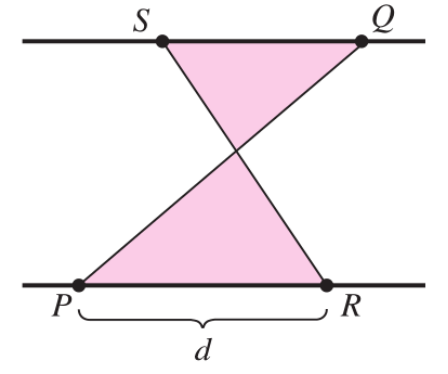
\includegraphics[scale=0.3]{pict1.PNG}
		\end{center}
		Titik $ R $ berjarak $ d $ dari $ P $. Seberapa jauh titik $ S $ dari $ Q $ ditempatkan agar jumlahan kedua luas daerah segitiga yang diarsir sekecil mungkin? Bagaimana juga jika luas daerah segitiga yang diarsir semaksimum mungkin?
		\item Sebuah tangki besar berbentuk kerucut harus dibuat dari potongan melingkar selembar logam berjari-jari 10 dengan cara membuang satu sektor dengan sudut pusat $ \theta $ dan kemudian mengelas sisi lurus lembaran sisa seperti pada gambar berikut.
		\begin{center}
			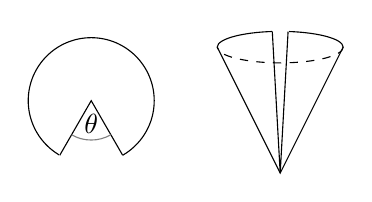
\begin{tikzpicture}[scale=0.4]
				%% GAMBAR 1 (LINGKARAN DENGAN SUDUT THETA) %%
				% Buat lingkaran
				\draw[name path=circle_A1] (-5, -0.2) arc (0:360:2);
				
				% Buat perpotongan antara rect_A1 dengan circle_A1 dan buat transparan
				\filldraw[name path=rect_A1, color=white]  (-8,-1) rectangle (-6,-2.5);
				\path[name intersections={of = rect_A1 and circle_A1, by={A1, B1}}];
				
				% Deklarasikan koordinat titik pusat circle_A1
				\coordinate (O) at (-7, -0.2);
				
				% Hubungkan antar titik untuk membuat lingkaran dengan sudut theta
				\draw (A1) -- (O) -- (B1);
				\draw pic[draw=gray, angle radius=5mm, "$ \theta $", angle eccentricity=0.6] {angle = A1--O--B1};
				%% AKHIR GAMBAR 1 %%
				
				%% GAMBAR 2 (KERUCUT) %%
				% Buat elips
				\draw[name path=half_ellipse_A2] (1, 1.5) arc (0:180:2 and 0.5);
				\draw[style=dashed, name path=half_ellipse_B2] (1, 1.5) arc (0:-180:2 and 0.5);
				
				% Buat perpotongan antara half_ellipse_A2 dengan rectA2 dan buat transparan
				\filldraw[name path=rectA2, color=white]  (-1.25,2.1) rectangle (-0.75,1.5);
				\path[name intersections={of = rectA2 and half_ellipse_A2, by={A2,B2}}];
				
				% Hubungkan antar titik untuk membuat kerucut
				\draw (A2) -- (-1, -2.5) -- (B2);
				\draw (-3, 1.5) -- (-1, -2.5) -- (1, 1.5);
				%% AKHIR GAMBAR 2 %%
			\end{tikzpicture}
		\end{center}
		Carilah $ \theta $ sehingga kerucut yang dihasilkan mempunyai volume sebesar mungkin.
		\item Sebuah jam dinding mempunyai jarum jam yang panjangnya $ h $ dan jarum menit yang panjangnya $ m $ dengan $ h \leq m $. Setiap waktu, sudut $ \theta $ antara jarum jam dan jarum menit ini selalu berubah. Kapankah ujung-ujung jarum jam dan jarum menit ini berpisah paling cepat?
		\item Dini pergi berlibur ke Pantai Biru Kersik. Di sana, Dini membuat beberapa bola pasir dan meletakkannya pada tepi pantai agar ombak dapat menyapu sedikit demi sedikit bola pasir yang telah ia buat. Dini mengamati bahwa setiap bola pasir yang tersapu oleh ombak akan terdeformasi pada suatu tingkat yang sebanding dengan luas permukaannya. Anggap bola pasir tetap mempertahankan bentuk bolanya secara sempurna hingga habis terkikis ombak. Jika salah satu bola pasir terdeformasi menjadi $ \dfrac{27}{64} $ dari volume semula dalam waktu satu jam, tentukan berapa lama bola pasir ini hingga habis terkikis ombak.
		\item Cari bilangan bulat positif $ j $ sedemikian sehingga untuk setiap polinomial $ \func{p}{x} $ dengan koefisien bilangan bulat dan untuk setiap bilangan bulat $ k $, $ \func{p^{\left(j\right)}}{k} $ habis dibagi 2021.
		\item Misalkan $ f $ terdiferensialkan. Jika kita menggunakan aproksimasi $ \func{f}{x + h} \approx \func{f}{x} + \func{f^{\prime}}{x}h $, maka galatnya adalah $ \func{\varepsilon}{h} = \func{f}{x + h} - \func{f}{x} - \func{f^{\prime}}{x}h $. Buktikan bahwa
		\[ \lim_{h \to 0}{\func{\varepsilon}{h}} = 0 \quad \mbox{dan} \quad \lim_{h \to 0}{\frac{\func{\varepsilon}{h}}{h}} = 0. \]
		\item Kesimpulan apa yang bisa diambil mengenai $ f $ dari informasi bahwa $ \func{f^{\prime}}{c} = \func{f^{\prime\prime}}{c} = 0 $ dan $ \func{f^{\prime\prime\prime}}{c} > 0 $?
		\item Diketahui fungsi $ f : \left(a, b\right) \to \mathbb{R} $ terdiferensial hingga tingkat berapapun di $ c \in \left(a, b\right) $. Tentukan nilai dari
		\[ \lim_{h \to 0}{\frac{\func{f}{c + h} - 2\func{f}{c} + \func{f}{c - h}}{h^{2}}}. \]
		\item Misalkan $ k $ suatu bilangan bulat positif tetap. Diketahui turunan ke-$ n $ dari $ \dfrac{1}{x^{k} - 1} $ memiliki bentuk $ \dfrac{\func{P_{n}}{x}}{\left(x^{k} - 1\right)^{n + 1}} $ dimana $ \func{P_{n}}{x} $ polinomial. Carilah nilai dari $ \func{P_{n}}{1} $.
		\item Diketahui fungsi $ f $ bernilai real terdefinisi pada $ \lkrb{1, +\infty} $ memenuhi $ \func{f}{1} = 1 $ dan $ \func{f^{\prime}}{x} = \dfrac{1}{x^{2} + \left(\func{f}{x}\right)^{2}} $. Tentukan nilai dari $ \ds{\lim_{x \to \infty}{\func{f}{x}}} $.
		\item Suatu titik pada $ \mathbb{R}^{2} $ disebut sebagai \textit{titik rasional} jika absis dan ordinatnya keduanya bilangan rasional. Jika $ S $ adalah himpunan semua titik rasional yang berada pada sisi suatu lingkaran di $ \mathbb{R}^{2} $ yang pusatnya bukan merupakan titik rasional, tentukan banyaknya anggota maksimum dari $ S $.
		\item Diketahui $ a < \dfrac{\pi}{2} $. Jika $ M < 1 $ dengan $ \left|\func{\cos}{x} - \func{\cos}{y}\right| \leq M\left|x - y\right| $ untuk setiap $ x, y \in \left[0, a\right] $, maka tentukanlah nilai $ M $.
		\item Misalkan $ f : \mathbb{R} \to \mathbb{R} $ terdiferensialkan hingga tingkat tiga sedemikian sehingga $ f $ memiliki setidaknya lima akar real berbeda. Buktikan bahwa $ f + 6f^{\prime} + 12f^{\prime\prime} + 8f^{\prime\prime\prime} $ memiliki setidaknya dua akar real berbeda.
		\item Berikan salah satu contoh fungsi kontinu $ f : \left[1, 4\right] \to \mathbb{R} $ dengan sifat setiap bilangan real $ K > 0 $, terdapat $ x, y \in \left[1, 4\right] $ yang memenuhi $ \left|\func{f}{x} - \func{f}{y}\right| > K\left|x - y\right| $.
		\item Cari semua fungsi terdiferensialkan $ f : \mathbb{R} \to \mathbb{R} $ sedemikian sehingga
		\[ \func{f^{\prime}}{x} = \frac{\func{f}{x + n} - \func{f}{x}}{n} \]
		untuk setiap bilangan real $ x $ dan setiap bilangan bulat positif $ n $.
		\item
		\begin{enumerate}
			\item Untuk setiap bilangan asli $ n $, buktikan bahwa terdapat polinomial $ \func{p_{n}}{x} $ dan $ \func{q_{n}}{x} $ sedemikian sehingga
			\[
				\begin{cases}
					\func{\sin}{n\theta} = \func{p_{n}}{\func{\tan}{\theta}}\func{\cos^{n}}{\theta}, \\
					\func{\cos}{n\theta} = \func{q_{n}}{\func{\tan}{\theta}}\func{\cos^{n}}{\theta}.
				\end{cases}
			\]
			\item Kemudian untuk $ n > 1 $, buktikan bahwa identitas berikut berlaku:
			\[
				\begin{cases}
					\func{\dfrac{\diff}{\diff{x}}p_{n}}{x} = n\func{q_{n - 1}}{x}, \\[5pt]
					\func{\dfrac{\diff}{\diff{x}}q_{n}}{x} = -n\func{p_{n - 1}}{x}.
				\end{cases}
			\]
		\end{enumerate}
		\item Suatu fungsi disebut sebagai fungsi \textit{terturunkan kontinu} jika fungsi tersebut terturunkan dan turunannya juga kontinu. Cari semua fungsi terturunkan kontinu tingkat dua $ f : \mathbb{R} \to \left(0, +\infty\right) $ yang memenuhi
		\[ \func{f^{\prime\prime}}{x}\func{f}{x} \geq 2\left(\func{f^{\prime}}{x}\right)^{2} \]
		untuk setiap bilangan real $ x $.
		\item Cari semua fungsi $ f : \mathbb{R^{+}} \to \mathbb{R^{+}} $ yang memenuhi $ \func{f}{x\func{f}{y}} = y\func{f}{x} $ untuk setiap bilangan real positif $ x, y $ dan $ \ds{\lim_{x \to \infty}{\func{f}{x}}} = 0 $.
		\item Diberikan fungsi $ f : \mathbb{R} \to \mathbb{R} $. Misalkan $ R_{f} $ daerah hasil fungsi $ f $. Buktikan atau bantah setiap pernyataan berikut ini:
		\begin{enumerate}
			\item Jika $ f $ kontinu dan $ R_{f} = \mathbb{R} $, maka $ f $ monoton.
			\item Jika $ f $ monoton dan $ R_{f} = \mathbb{R} $, maka $ f $ kontinu.
			\item Jika $ f $ monoton dan $ f $ kontinu, maka $ R_{f} = \mathbb{R} $.
		\end{enumerate}
		\item Misalkan fungsi $ f : \left[a, b\right] \to \mathbb{R} $ kontinu pada $ \left[a, b\right] $ dan terdiferensialkan pada $ \left(a, b\right) $. Asumsikan $ f $ memiliki tak hingga banyaknya akar, tetapi tidak ada $ x \in \left(a, b\right) $ dengan $ \func{f}{x} = \func{f^{\prime}}{x} = 0 $.
		\begin{enumerate}
			\item Buktikan bahwa $ \func{f}{a}\func{f}{b} = 0 $.
			\item Begikan contoh fungsi yang memenuhi pada $ \left[0, 1\right] $.
		\end{enumerate}
		\item Misalkan $ f : \mathbb{R} \to \mathbb{R} $ fungsi kontinu. Suatu titik $ x $ disebut sebgai \textit{titik bayangan} jika terdapat suatu titik $ y \in \mathbb{R} $ dengan $ y > x $ sedemikian sehingga $ \func{f}{y} > \func{f}{x} $. Misalkan $ a < b $ bilangan real dan asumsikan bahwa
		\begin{enumerate}[label=$\bullet$]
			\item Semua titik pada interval buka $ \left(a, b\right) $ merupakan titik bayangan;
			\item $ a $ dan $ b $ bukan titik bayangan.
		\end{enumerate}
		Buktikan bahwa
		\begin{enumerate}
			\item $ \func{f}{x} \leq \func{f}{b} $ untuk setiap $ a < x < b $;
			\item $ \func{f}{a} = \func{f}{b} $.
		\end{enumerate}
		\item Misalkan $ f : \mathbb{R} \to \mathbb{R} $ fungsi yang terdiferensialkan tingkat dua. Asumsikan $ \func{f}{0} = 0 $. Buktikan bahwa terdapat $ \xi \in \left(-\dfrac{\pi}{2}, \dfrac{\pi}{2}\right) $ sedemikian sehingga
		\[ \func{f^{\prime\prime}}{\xi} = \func{f}{\xi}\left(1 + 2\func{\tan^{2}}{\xi}\right). \]
		\item Misalkan $ \func{f}{x} = \dfrac{\func{\sin}{x}}{x} $ untuk $ x > 0 $ dan misalkan $ n $ bilangan bulat positif. Buktikan bahwa
		\[ \left|\func{f^{\left(n\right)}}{x}\right| < \frac{1}{n + 1}. \]
		\item Misalkan $ f $ dan $ g $ fungsi bernilai real yang terdefinisi pada interval buka yang mengandung 0 dengan $ g $ taknol dan kontinu pada 0. Jika $ fg $ dan $ f/g $ terdiferensialkan di 0, haruskah $ f $ juga terdiferensialkan di 0?
		\item Cari semua fungsi terdiferensialkan $ f : \left(0, +\infty\right) \to \left(0, +\infty\right) $ sehingga terdapat bilangan real positif $ a $ yang memenuhi
		\[ \func{f^{\prime}}{\frac{a}{x}} = \frac{x}{\func{f}{x}} \]
		untuk setiap bilangan real $ x > 0 $.
		\item Suatu fungsi disebut sebagai fungsi \textit{terturunkan kontinu} jika fungsi tersebut terturunkan dan turunannya juga kontinu. Apakah terdapat fungsi terturunkan kontinu $ f : \mathbb{R} \to \mathbb{R} $ sedemikian sehingga untuk setiap $ x \in \mathbb{R} $, kita punyai $ \func{f}{x} > 0 $ dan $ \func{f^{\prime}}{x} = \func{\left(f \circ f\right)}{x} $?
		\item Misalkan $ f $ fungsi real pada garis bilangan real dengan turunan ketiga kontinu. Buktikan bahwa terdapat suatu titik $ a \in \mathbb{R} $ sedemikian sehingga
		\[ \func{f}{a} \cdot \func{f^{\prime}}{a} \cdot \func{f^{\prime\prime}}{a} \cdot \func{f^{\prime\prime\prime}}{a} \geq 0. \]
		\item Misalkan $ \func{p}{x} $ polinomial taknol berderajat kurang dari 2021 dan tidak memiliki faktor nonkonstan dengan $ x^{3} - x $. Misalkan juga
		\[ \func{\frac{\diff^{2021}}{\diff x^{2021}}}{\frac{\func{p}{x}}{x^{3} - x}} = \frac{\func{f}{x}}{\func{g}{x}} \]
		untuk suatu polinomial $ \func{f}{x} $ dan $ \func{g}{x} $. Cari derajat terkecil yang mungkin dari $ \func{f}{x} $.
		\item* Diketahui $ \Omega $ adalah koleksi semua fungsi $ f : \mathbb{R} \to \mathbb{R} $ yang memenuhi
		\[ \left|\func{f}{x} - \func{f}{t}\right| \leq \left|x - t\right|^{4} \]
		untuk setiap $ x, t \in \mathbb{R} $. Buktikan bahwa untuk setiap $ f \in \Omega $, $ f $ merupakan fungsi terbatas pada $ \mathbb{R} $. Artinya, terdapat suatu $ c \in \mathbb{R} $ sedemikian sehingga berlaku $ -c \leq \func{f}{x} \leq c $ untuk setiap bilangan real $ x $.
		\item* Misalkan $ f $ fungsi real dengan turunan ketiga kontinu sedemikian sehingga $ \func{f}{x} $, $ \func{f^{\prime}}{x} $, $ \func{f^{\prime\prime}}{x} $, dan $ \func{f^{\prime\prime\prime}}{x} $ semuanya bernilai positif untuk setiap bilangan real $ x $. Asumsikan $ \func{f^{\prime\prime\prime}}{x} \leq \func{f}{x} $ untuk setiap bilangan real $ x $. Buktikan bahwa $ \func{f^{\prime}}{x} < 2\func{f}{x} $ untuk setiap bilangan real $ x $.
		\item* Buktikan bahwa terdapat tepat satu fungsi $ f : \mathbb{R^{+}} \to \mathbb{R}^{+} $ sedemikian sehingga $ \func{f}{\func{f}{x}} = 6x - \func{f}{x} $ dan $ \func{f}{x} > 0 $ untuk setiap $ x > 0 $.
		\item* Cari semua fungsi monoton murni $ f : \left(0, +\infty\right) \to \left(0, +\infty\right) $ sedemikian sehingga $ \func{f}{\dfrac{x^{2}}{\func{f}{x}}} \equiv x $.
		\item* Diketahui fungsi $ f : \mathbb{R} \to \mathbb{R} $ terdiferensial hingga tingkat 2. Jika terdapat bilangan real positif $ A $ dan $ B $ dengan sifat $ \left|\func{f}{x}\right| \leq A $ dan $ \left|\func{f^{\prime\prime}}{x}\right| \leq B $ untuk setiap $ x \in \mathbb{R} $, buktikan bahwa
		\[ \left|\func{f^{\prime}}{0}\right| \leq 2\sqrt{AB}. \]
		\item* Jika fungsi $ f : \left[0, 1\right] \to \left[0, 1\right] $ memenuhi $ \left|\func{f}{x} - \func{f}{y}\right| \leq \left|x - y\right| $ untuk setiap $ x, y \in \left[0, 1\right] $, buktikan bahwa $ F = \set{x \in \left[0, 1\right]}{\func{f}{x} = x} $ merupakan \textit{singleton} atau interval. \\
		\textit{Catatan: singleton adalah himpunan dengan tepat satu anggota.}
		\item* Jika fungsi $ f : \mathbb{R} \to \mathbb{R} $ terdiferensial dan terdapat $ c \in \mathbb{R} $ dengan $ \ds{\lim_{x \to \infty}{\func{f^{\prime}}{x}}} = c $, tunjukkan bahwa
		\[ \lim_{x \to c}{\frac{\func{f}{x}}{x}} = c. \]
		\item* Misalkan $ f : \mathbb{R} \to \mathbb{R} $ adalah fungsi yang turunan tingkat duanya ada dan $ \func{f^{\prime\prime}}{x} < 0 $ untuk setiap bilangan real $ x $. Buktikan bahwa bangun yang dibentuk dari titik-titik $ \left(1, \func{f}{1}\right) $, $ \left(2, \func{f}{2}\right) $, $ \left(3, \func{f}{3}\right) $, dan $ \left(4, \func{f}{4}\right) $ bukan merupakan jajar genjang.
		\item* Buktikan bahwa tidak terdapat fungsi $ f : \mathbb{R} \to \mathbb{R} $ dengan $ \func{f}{0} > 0 $ sedemikian sehingga
		\[ \func{f}{x + y} \geq \func{f}{x} + y\func{f}{\func{f}{x}} \quad \mbox{untuk setiap} \quad x, y \in \mathbb{R}. \]
		\item* Misalkan $ f : \mathbb{R} \to \mathbb{R} $ fungsi yang terdiferensialkan hingga tingkat dua dan memenuhi $ \func{f}{0} = 2 $, $ \func{f^{\prime}}{0} = -2 $, dan $ \func{f}{1} = 1 $. Buktikan bahwa terdapat bilangan real $ \xi \in \left(0, 1\right) $ sedemikian sehingga
		\[ \func{f}{\xi} \cdot \func{f^{\prime}}{\xi} + \func{f^{\prime\prime}}{\xi} = 0. \]
		\item* Buktikan bahwa jika $ f : \mathbb{R} \to \mathbb{R} $ merupakan fungsi yang terdiferensialkan hingga tingkat dua, maka terdapat bilangan real $ \xi \in \left(-1, 1\right) $ sedemikian sehingga
		\[ \frac{\func{f^{\prime\prime\prime}}{\xi}}{6} = \frac{\func{f}{1} - \func{f}{-1}}{2} - \func{f^{\prime}}{0}. \]
		\item* Buktikan bahwa jika fungsi $ f $ mempunyai turunan di setiap $ x \in \left[a, b\right] $, maka untuk setiap $ \gamma $ di antara $ \func{f^{\prime}}{a} $ dan $ \func{f^{\prime}}{b} $, terdapat $ c \in \left[a, b\right] $ dengan $ \func{f^{\prime}}{c} = \gamma $.
		\item* Diketahui fungsi $ f: \mathbb{R} \to \mathbb{R} $ kontinu dan surjektif. Jika untuk setiap $ y \in \mathbb{R} $, cacah anggota himpunan $ \set{x \in \mathbb{R}}{\func{f}{x} = y} $ paling banyak dua, buktikan bahwa $ f $ monoton.
		\item* Apakah terdapat fungsi naik murni $ f : \mathbb{R} \to \mathbb{R} $ sedemikian sehingga $ \func{f^{\prime}}{x} = \func{f}{\func{f}{x}} $ untuk setiap bilangan real $ x $?
		\item* Misalkan $ a $ dan $ b $ bilangan real yang berada dalam interval $ \left(0, \dfrac{1}{2}\right) $ serta misalkan $ g $ fungsi kontinu bernilai real sedemikian sehingga $ \func{g}{\func{g}{x}} = a\func{g}{x} + bx $ untuk setiap bilangan real $ x $. Buktikan bahwa $ \func{g}{x} = cx $ untuk suatu konstanta $ c \in \mathbb{R} $.
		\item* Misalkan $ P $ polinomial berderajat $ n $ yang memiliki koefisien real dan akar-akar yang juga real. Buktikan bahwa untuk setiap bilangan real $ x $ berlaku
		\[ \left(n - 1\right)\left(\func{P^{\prime}}{x}\right)^{2} \geq n\func{P}{x}\func{P^{\prime\prime}}{x}. \]
		Kapankah kesamaan tercapai?
		\item** Suatu fungsi disebut sebagai fungsi \textit{terturunkan kontinu} jika fungsi tersebut terturunkan dan turunannya juga kontinu. Cari semua fungsi terturunkan kontinu $ f : \mathbb{R} \to \mathbb{R} $ sedemikian sehingga untuk setiap bilangan rasional $ q $, nilai dari $ \func{f}{q} $ juga rasional dan memiliki penyebut sama dengan penyebut $ q $ (disini, $ q $ dalam bentuk yang paling sederhana).
		\item** Misalkan $ f : \mathbb{R} \to \mathbb{R} $ fungsi terdiferensialkan hingga tingkat berapa pun yang memenuhi $ \func{f}{0} = 0 $, $ \func{f}{1} = 1 $, dan $ \func{f}{x} \geq 0 $ untuk setiap $ x \in \mathbb{R} $. Buktikan bahwa terdapat bilangan bulat positif $ n $ dan bilangan real $ r $ sedemikian sehingga $ \func{f^{\left(n\right)}}{x} < 0 $.
		\item** Untuk setiap bilangan real $ \alpha $, definisikan fungsi $ f_{\alpha} $ sebagai $ \func{f_{\alpha}}{x} = \floor{\alpha x} $. Misalkan $ n $ bilangan bulat positif. Buktikan bahwa terdapat $ \alpha $ sedemikian sehingga untuk $ 1 \leq k \leq n $ berlaku
		\[ \func{f_{\alpha}^{k}}{n^{2}} = n^{2} - k - \func{f_{\alpha^{k}}}{n^{2}} \]
		dimana $ \floor{x} $ dinotasikan sebagai bilangan bulat terbesar yang kurang dari atau sama dengan $ x $ dan $ f_{\alpha}^{k} \coloneqq f_{\alpha} \circ \cdots \circ f_{\alpha} $.
		\item** Misalkan $ f \ne 0 $ polinomial dengan koefisien real. Definisikan barisan polinomial $ f_{0}, f_{1}, f_{2}, \dots $ dengan $ f_{0} = f $ dan $ f_{n + 1} = f_{n} + f_{n}^{\prime} $ untuk setiap $ n \geq 0 $. Buktikan bahwa terdapat bilangan bulat positif $ N $ sedemikian sehingga untuk setiap $ n \geq N $, semua akar $ f_{n} $ bernilai real.
	\end{enumerate}
\end{document}
